\question[6]行驶中的汽车如果发生剧烈碰撞,车内的安全气囊会被弹出并瞬间充满气体.若碰撞后汽车的速度在很短时间内减小为零,关于安全气囊在此过程中的作用,下列说法正确的是\key{D}
\fourchoices{增加了司机单位面积的受力大小}{减少了碰撞前后司机动量的变化量}{将司机的动能全部转换成汽车的动能}{延长了司机的受力时间并增大了司机的受力面积}
\begin{solution}{4cm}

\end{solution}



\question[6]火星的质量约为地球质量的$1/10,$半径约为地球半径的$1/2,$则同一物体在火星表面与在地球表面受到的引力的比值约为\key{B}
\fourchoices{$0.2$}{$0.4$}{$2.0$}{$2.5$}
\begin{solution}{4cm}

\end{solution}



\question[6]如图,一同学表演荡秋千.已知秋千的两根绳长均为$10m,$该同学和秋千踏板的总质量约为$50kg.$绳的质量忽略不计,当该同学荡到秋千支架的正下方时,速度大小为$8m/s,$此时每根绳子平均承受的拉力约为\key{B}
\begin{center}
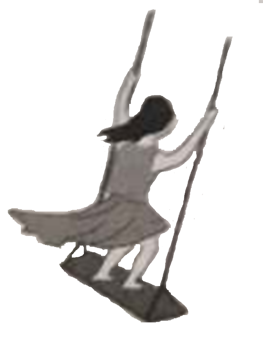
\includegraphics[]{img/image1.png}
\end{center}

\fourchoices{$200N$}{$400N$}{$600N$}{$800N$}
\begin{solution}{4cm}

\end{solution}


\newpage
\question[6]图(a)所示的电路中,K与L间接一智能电源,用以控制电容器C两端的电压$U_C.$如果$U_C$随时间t的变化如图(b)所示,则下列描述电阻R两端电压$U_R$随时间t变化的图像中,正确的是\key{A}
\begin{center}
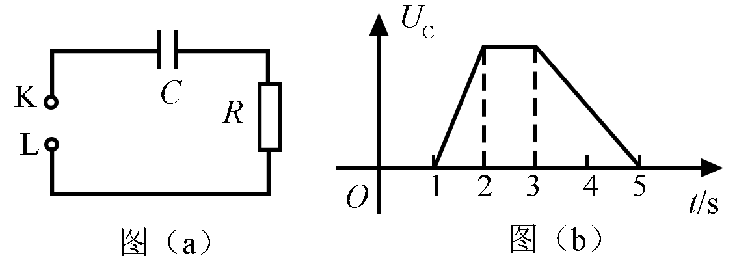
\includegraphics[width=8cm]{img/image2.png}
\end{center}
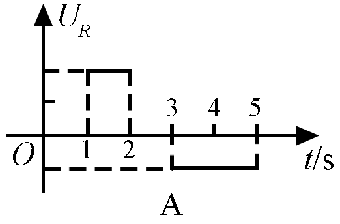
\includegraphics[width=3.5cm]{img/image3.png}
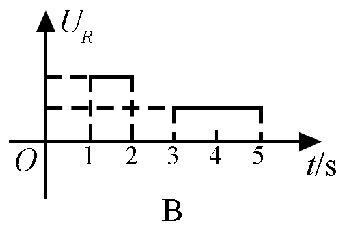
\includegraphics[width=3.5cm]{img/image4.png}
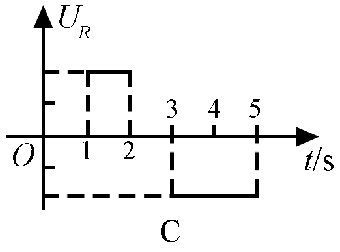
\includegraphics[width=3.5cm]{img/image5.png}
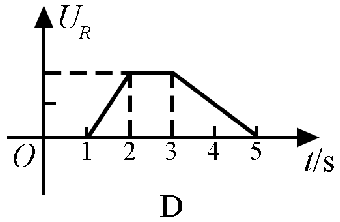
\includegraphics[width=3.5cm]{img/image6.png}

\begin{solution}{4cm}

\end{solution}



\question[6]一匀强磁场的磁感应强度大小为B,方向垂直于纸面向外,其边界如图中虚线所示$,ab$为半圆$,ac$、$bd$与直径ab共线$,ac$间的距离等于半圆的半径.一束质量为m、电荷量为$q(q>0)$的粒子,在纸面内从c点垂直于ac射入磁场,这些粒子具有各种速率.不计粒子之间的相互作用.在磁场中运动时间最长的粒子,其运动时间为\key{C}
\begin{center}
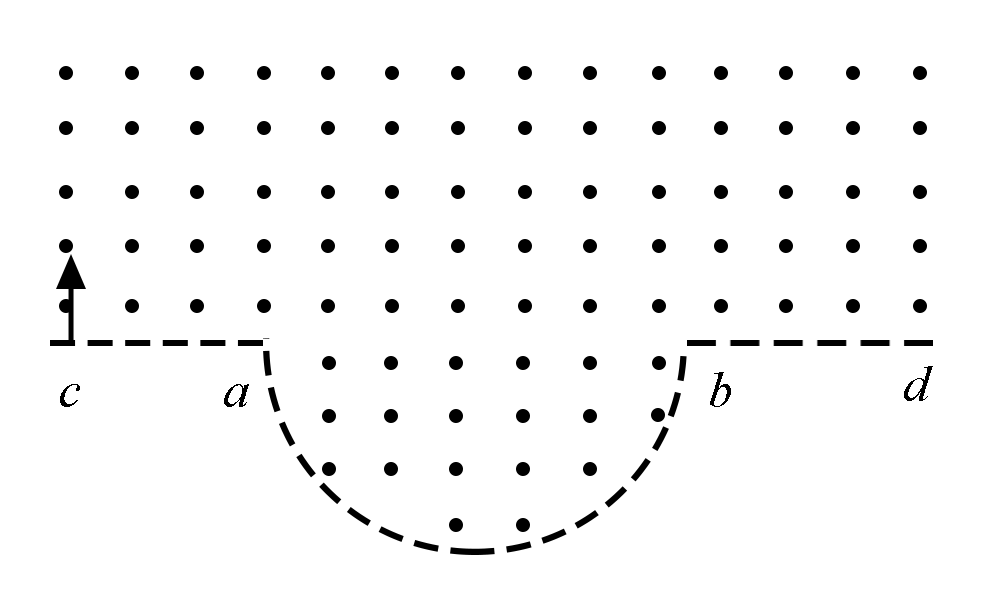
\includegraphics[]{img/image7.png}
\end{center}

\fourchoices{$\frac{7\pi m}{6qB}$}{$\frac{5\pi m}{4qB}$}{$\frac{4\pi m}{3qB}$}{$\frac{3\pi m}{2qB}$}
\begin{solution}{4cm}

\end{solution}



\question[6]下列核反应方程中$,X_1,X_2,X_3,X_4$代表α粒子的有\key{BD}
\fourchoices{$_1^2H+_1^2H→_0^10^n+X_1$}{$^{2}_{1}H+_{1}^{3}H\rightarrow_{0}^{1}n+X_{2}$}{$_{92}^{235}U+_{0}^{1}n\rightarrow_{56}^{144}Ba+\frac{89}{36}Kr+3X_{3}$}{$_{0}^{1}n+\frac{6}{3}Li\rightarrow_{1}^{3}H+X_{4}$}
\begin{solution}{4cm}

\end{solution}


\newpage
\question[6]一物块在高$3.0m$、长$5.0m$的斜面顶端从静止开始沿斜面下滑,其重力势能和动能随下滑距离s的变化如图中直线\uppercase\expandafter{\romannumeral1}、\uppercase\expandafter{\romannumeral2 }所示,重力加速度取$10m/s^2.$则\key{AB}
\begin{center}
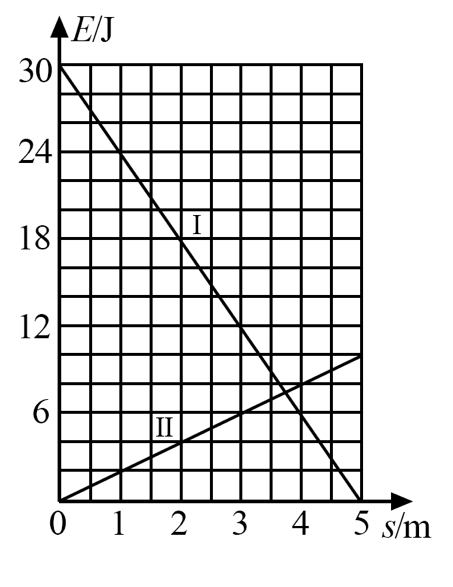
\includegraphics[]{img/image8.png}
\end{center}

\fourchoices{物块下滑过程中机械能不守恒}{物块与斜面间的动摩擦因数为$0.5$}{物块下滑时加速度的大小为$6.0m/s^2$}{当物块下滑$2.0m$时机械能损失了$12J$}
\begin{solution}{4cm}

\end{solution}



\question[6]如图,U形光滑金属框$abcd$置于水平绝缘平台上$,ab$和dc边平行,和bc边垂直$.ab$、$dc$足够长,整个金属框电阻可忽略.一根具有一定电阻的导体棒MN置于金属框上,用水平恒力F向右拉动金属框,运动过程中,装置始终处于竖直向下的匀强磁场中$,MN$与金属框保持良好接触,且与bc边保持平行.经过一段时间后\key{BC}
\begin{center}
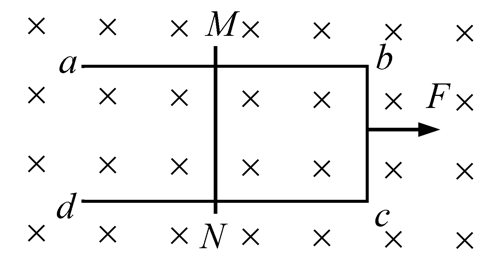
\includegraphics[]{img/image9.png}
\end{center}

\fourchoices{属框的速度大小趋于恒定值}{属框的加速度大小趋于恒定值}{体棒所受安培力的大小趋于恒定值}{体棒到金属框bc边的距离趋于恒定值}
\begin{solution}{4cm}

\end{solution}
\newpage


